\documentclass[conference]{IEEEtran}
% Energy-Harvester-Powered PMU -- two-stage CMOS error amplifier (gpdk180).
% Figures (same directory): fig_block.png fig_sch.png fig_dcop.png
% fig_gain.png fig_pm.png fig_cmrr.png fig_tran.png
% Compile: pdflatex pmu_report.tex  (run from this directory, or Overleaf)
\usepackage{graphicx}
\usepackage{booktabs}
\usepackage{siunitx}
\usepackage[hidelinks]{hyperref}
\sisetup{detect-all}

\begin{document}

\title{Design of an Energy-Harvester-Powered Power Management Unit for
Low-Power Applications Using 0.18~\si{\micro\metre} CMOS Technology in
Cadence Virtuoso}

\author{\IEEEauthorblockN{Purvesh Vaghela (23BEC201) \qquad Utsav Raiyani (23BEC199)}
\IEEEauthorblockA{Department of Electronics and Communication Engineering,
Institute of Technology, Nirma University\\
Mentor: Prof.\ Purvi Patel --- Course: Research Methodology \& Seminar}}

\maketitle

\begin{abstract}
Battery-less sensor nodes and Internet of Things (IoT) devices depend on
energy harvested from the environment, but harvested sources such as small
solar cells deliver low and fluctuating voltages, approximately
0.3--1~\si{\volt}, which cannot power electronic loads directly. A power
management unit (PMU) is therefore required to condition, store and regulate
the harvested energy. This report presents the architecture of a proposed
solar energy-harvesting PMU and the design and standalone characterization of
its first implemented block: a two-stage CMOS operational amplifier intended
as the error amplifier of a future low-dropout (LDO) regulator. The amplifier
uses a PMOS differential input pair with a current-mirror load, a
common-source second stage, and Miller compensation with a series nulling
resistor. It was designed by square-law hand sizing and simulated in Cadence
Virtuoso using the gpdk180 process at a \SI{1.8}{\volt} supply and a
\SI{0.5}{\volt} input common mode. The simulated amplifier achieves
approximately \SI{70.5}{\decibel} open-loop gain, \SI{1.629}{\mega\hertz}
unity-gain bandwidth, \ang{51.8} phase margin, \SI{87.8}{\decibel} CMRR at
\SI{10}{\hertz}, and a reported ADE power figure of \SI{4.73}{\micro\watt} at
\SI{3.27}{\micro\ampere} supply current. The phase margin falls short of the
\ang{60} design guideline, and the complete PMU --- LDO, reference,
boost/conditioning stage and voltage monitor --- remains proposed rather than
implemented. The report separates verified amplifier results from proposed
LDO values and sets out the verification plan for the remaining blocks.
\end{abstract}

\begin{IEEEkeywords}
Energy harvesting, power management unit, low-dropout regulator, error
amplifier, two-stage CMOS operational amplifier, Miller compensation,
0.18~\si{\micro\metre} CMOS.
\end{IEEEkeywords}

\section{Introduction}
Wireless sensor networks and IoT deployments increasingly favour nodes that
operate without battery replacement, placing the supply burden on energy
harvested from the environment. Among ambient sources, small solar cells
offer comparatively high power density and natural CMOS compatibility; this
motivated the solar-harvesting PMU of Patel et al.\ in 0.18~\si{\micro\metre}
CMOS, the principal reference for this project \cite{patel2017}.

Harvested electrical energy is, however, poorly suited to direct use. The
project presentation models two series solar cells that deliver roughly
0.3--1~\si{\volt} depending on illumination, and the available power varies
with the environment. A PMU bridges this gap: it conditions the input, stores
energy, generates a reference, regulates the supply seen by the load, and can
disconnect the load when stored energy is insufficient. Within such a PMU,
the regulation duty falls on a linear LDO stage, whose accuracy and stability
are set largely by its error amplifier \cite{rincon1998,razavi}. The error
amplifier compares a divided copy of the output with a reference and drives
the gate of a PMOS pass transistor, so its gain, bandwidth, phase margin and
quiescent current directly determine the regulation quality and the power
overhead of the whole unit.

This project therefore begins the PMU design with its most
performance-critical analog block. A two-stage CMOS operational amplifier was
designed by square-law hand analysis, implemented in Cadence Virtuoso on the
generic 0.18~\si{\micro\metre} process design kit (gpdk180), and
characterized with the Spectre simulator. The 0.18~\si{\micro\metre} node was
selected because it is the technology of the reference PMU \cite{patel2017},
offers well-characterized \SI{1.8}{\volt} devices with adequate headroom for
a two-stage topology, and is the process available in the institute's Cadence
environment. This report documents the architecture, sizing, simulation
methodology and measured standalone results of the amplifier, and presents
the proposed --- not yet implemented --- LDO and PMU integration plan.

\section{Problem Statement, Objectives and Scope}
\textbf{Problem statement.} To design an energy harvester-powered power
management unit for low-power applications using 0.18~\si{\micro\metre} CMOS
technology in Cadence Virtuoso, converting a low and fluctuating harvested
input into a regulated supply suitable for low-power loads such as sensor
nodes.

The measurable objectives, with their verification methods and present
status, are collected in Table~\ref{tab:obj}. Objectives 1--3 concern the
error amplifier and are complete at schematic level; objectives 4--7 define
the remaining system work. The scope completed so far is the standalone
amplifier: schematic entry, DC operating-point verification, AC gain/phase,
CMRR, transient and slew-rate simulation. The proposed scope --- LDO closure
around a PMOS pass device, reference, input conditioning or boost stage,
storage, and voltage monitoring --- is specified but unverified.

\begin{table}[!t]
\caption{Project Objectives and Verification Criteria}
\label{tab:obj}
\centering\footnotesize
\begin{tabular}{@{}clll@{}}
\toprule
\# & Objective / requirement & Verification & Status \\
\midrule
1 & Two-stage error amp in gpdk180; all devices & DC operating & Done (all \\
  & saturated at $V_{DD}$=\SI{1.8}{\volt}, $V_{ICM}$=\SI{0.5}{\volt} & point & region 2) \\
2 & $A_v{\ge}60$~dB; GBW 10--2000~kHz; & AC / CMRR & Done (70.5 dB; \\
  & CMRR${\ge}80$~dB & analyses & 1.629 MHz; 87.8 dB) \\
3 & PM${\ge}$\ang{60}; SR${\ge}0.1$~V/\si{\micro\second}; & AC phase, tran., & Partial --- PM \\
  & $P{<}10$--100~\si{\micro\watt} & ADE power & \ang{51.8} below \ang{60} \\
4 & LDO closure: $V_{out}$=\SI{1.2}{\volt} from & DC, sweeps, & Proposed --- \\
  & $V_{ref}$=\SI{0.5}{\volt} at $\le$\SI{100}{\micro\ampere} & loop gain & not simulated \\
5 & Voltage reference \SI{0.5}{\volt}, low power & DC, temp.\ sweep & Proposed \\
6 & Harvest interface / boost + storage & System transient & Proposed \\
  & from 0.3--1~\si{\volt} source & & \\
7 & Voltage monitor and load control & System transient & Proposed \\
\bottomrule
\end{tabular}
\end{table}

\section{Related Work}
Patel, Mishra and Nagchoudhuri integrate on-chip solar cells with a
\SI{36}{\nano\watt} PMU in 0.18~\si{\micro\metre} CMOS, using a subthreshold
cascoded error amplifier inside an LDO; their work demonstrates the
feasibility of full integration but accepts modest amplifier gain
($\approx$\SI{46}{\decibel}) and bandwidth as the price of nanowatt operation
\cite{patel2017}. The present project deliberately diverges by biasing the
amplifier in strong/moderate inversion from a \SI{1.8}{\volt} rail, trading
microwatt quiescent power for higher, more predictable gain.
Rinc\'on-Mora and Allen established the canonical low-quiescent-current LDO
analysis --- pass-device sizing, loop stability with the output capacitor and
its equivalent series resistance (ESR) --- that the proposed LDO stage
follows \cite{rincon1998}. For the amplifier itself, the two-stage
Miller-compensated topology and the nulling-resistor technique for cancelling
the right-half-plane (RHP) zero are standard results covered in Razavi and in
Gray et al.\ \cite{razavi,gray}; Allen and Holberg give the square-law design
procedure used for hand sizing \cite{allen}. On the system side, Seok et al.\
demonstrate a picowatt 2-transistor \SI{0.5}{\volt} reference suitable for
harvesting PMUs \cite{seok2012}, and Seeman and Sanders provide the analysis
framework for the switched-capacitor conversion stage that the
0.3--1~\si{\volt} source will require \cite{seeman2008}.
Table~\ref{tab:lit} compares these works; NR marks values not reported by the
cited source.

\begin{table}[!t]
\caption{Literature Comparison (NR = Not Reported in the Cited Source)}
\label{tab:lit}
\centering\scriptsize
\begin{tabular}{@{}llllll@{}}
\toprule
Ref. & Tech. & Architecture & Power & Gain / BW & Limitation \\
\midrule
\cite{patel2017} & 0.18~\si{\micro\metre} & Solar PMU: LDO + & 36 nW & 46.39 dB / & Subthreshold: \\
 & & subthr.\ casc.\ amp & (PMU) & 206 kHz & low gain, slow \\
\cite{rincon1998} & 2~\si{\micro\metre} & Low-dropout & NR & NR & Older node; \\
 & BiCMOS & regulator & & & discrete $C_{out}$ \\
\cite{seok2012} & 0.13~\si{\micro\metre} & 2-T voltage ref. & pW & --- & Untrimmed \\
 & & \SI{0.5}{\volt} & & & accuracy \\
\cite{seeman2008} & theory & SC DC--DC analysis & --- & --- & No silicon \\
This work & 0.18~\si{\micro\metre} & Two-stage error & 4.73~\si{\micro\watt} & 70.5 dB / & PM \ang{51.8}; \\
 & (gpdk180) & amp for PMU LDO & (def.\ pending) & 1.629 MHz & system proposed \\
\bottomrule
\end{tabular}
\end{table}

\section{Proposed PMU Architecture}
\begin{figure}[!t]
\centering
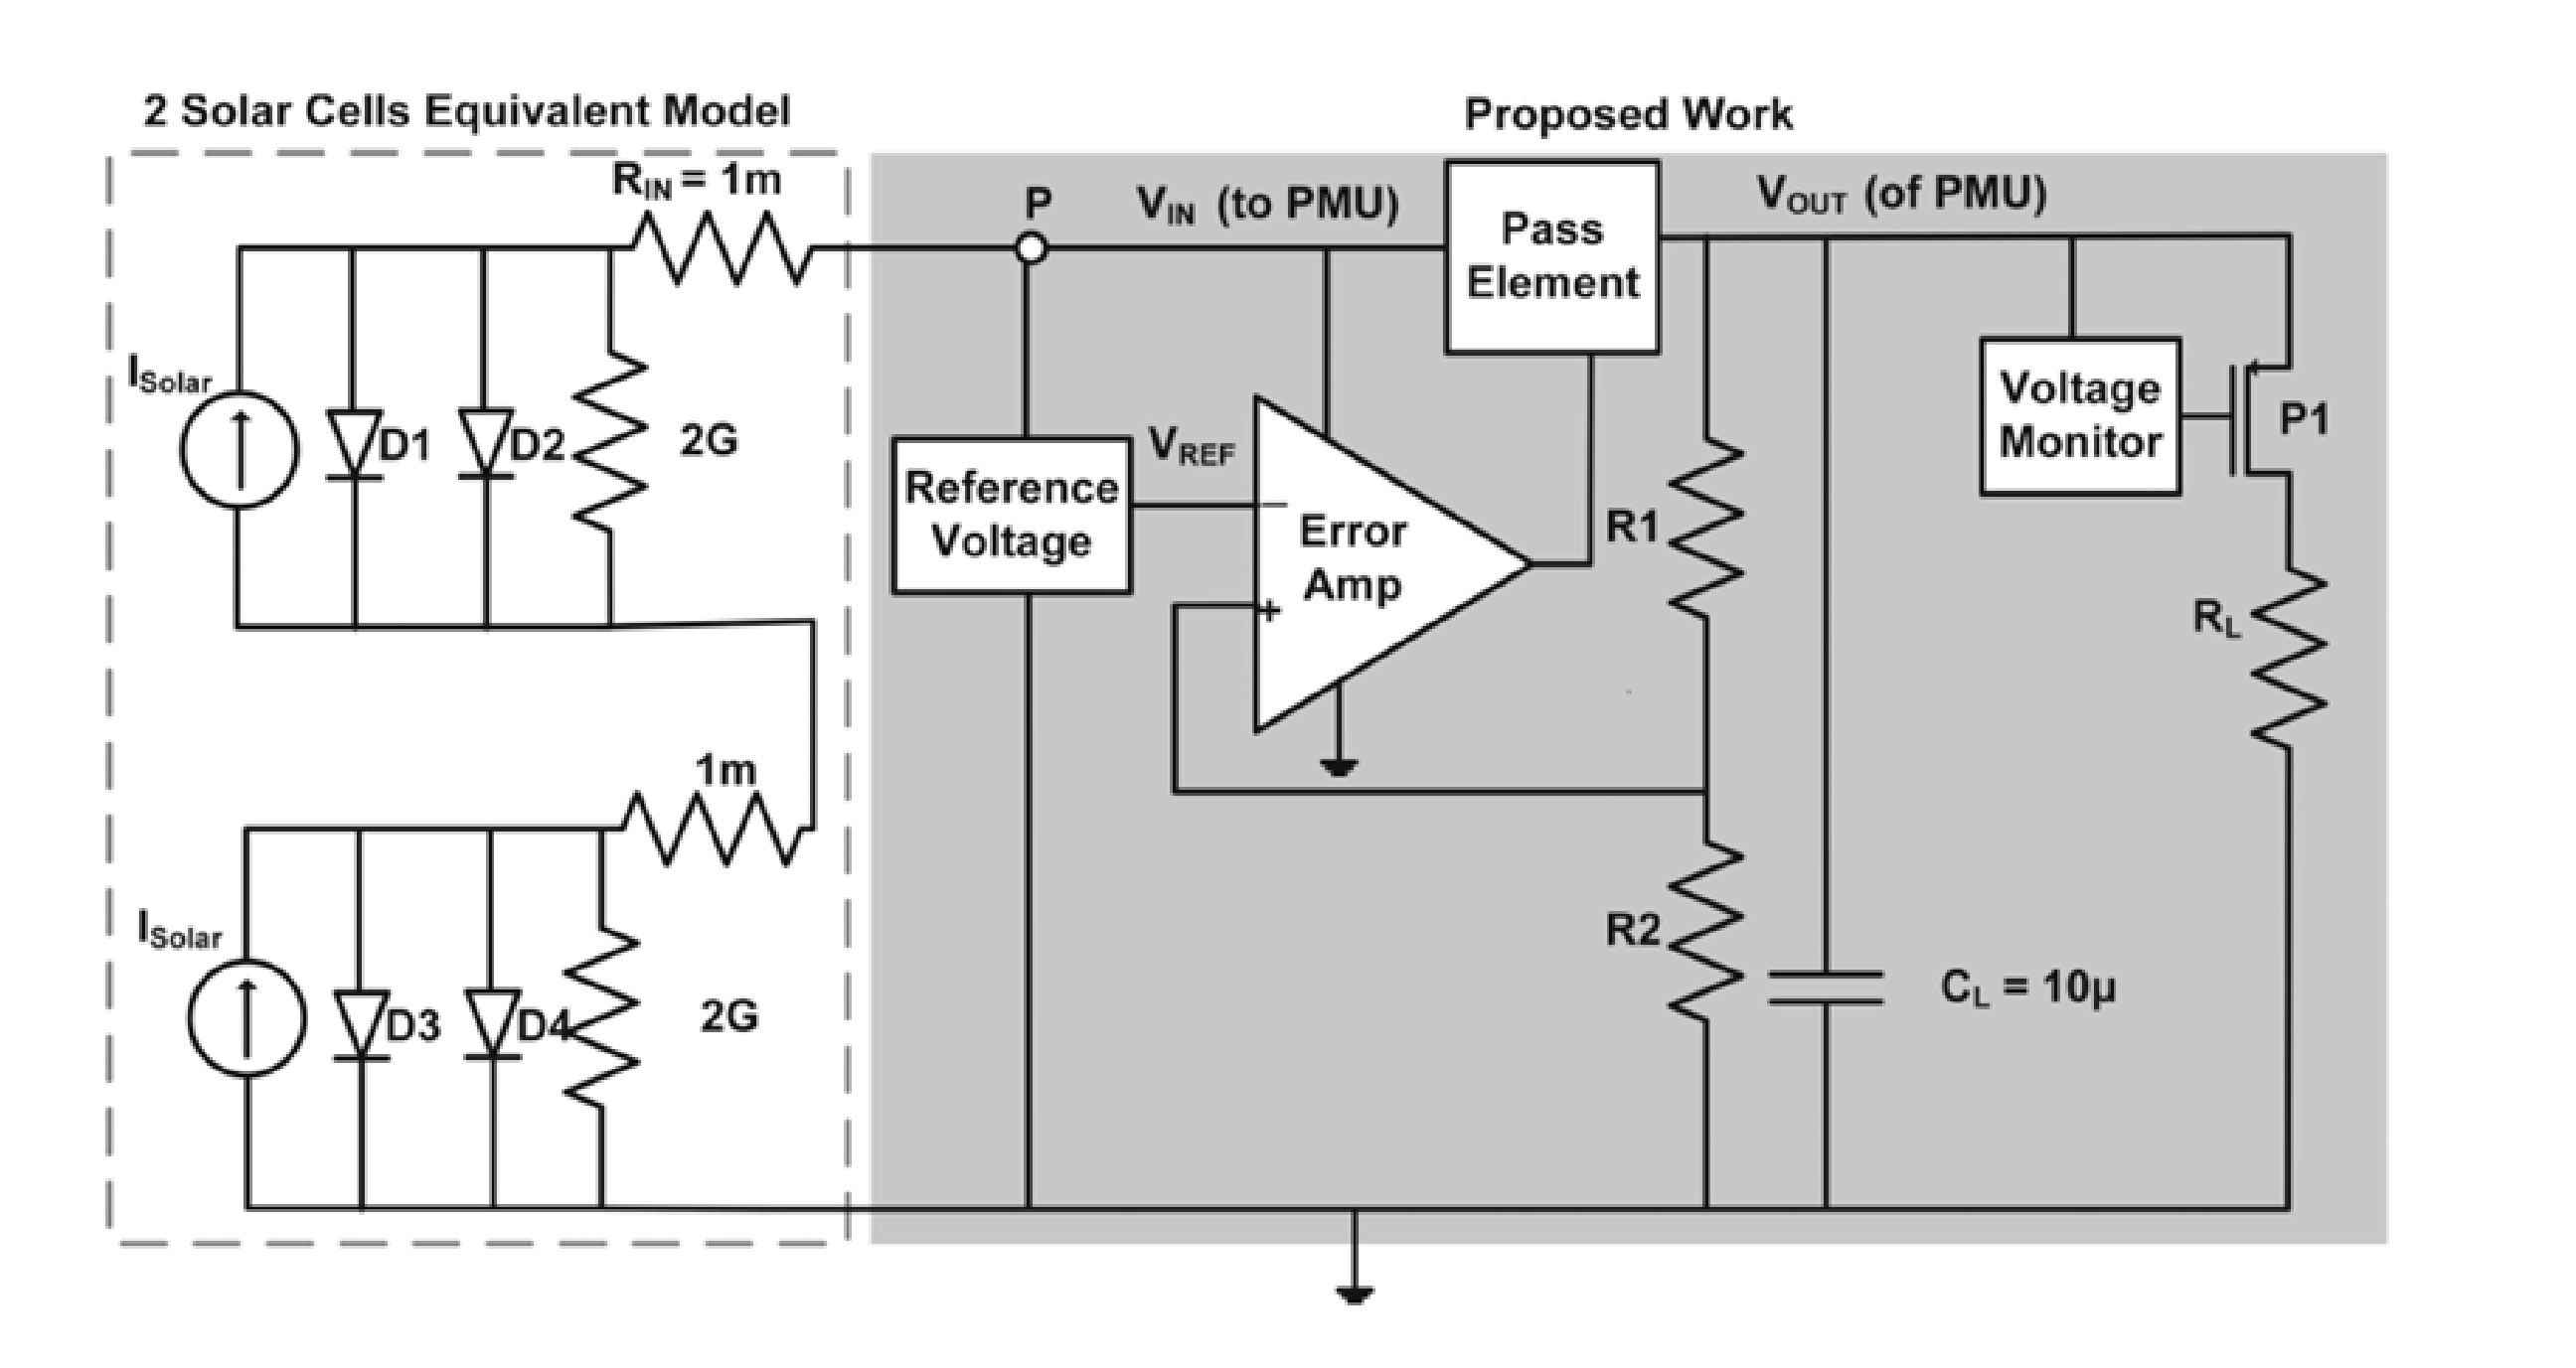
\includegraphics[width=0.95\columnwidth]{fig_block.png}
\caption{Proposed PMU block diagram from the project presentation: solar-cell
equivalent model (left) feeding the proposed regulation chain --- reference,
error amplifier, pass element, $R_1$/$R_2$ feedback divider,
$C_L$=\SI{10}{\micro\farad} output capacitor, voltage monitor and load switch
P1. Only the error amplifier is implemented to date.}
\label{fig:block}
\end{figure}

Energy and signal flow proceed left to right in Fig.~\ref{fig:block}. The
harvester (two series solar cells, each an $I_{solar}$ source with diodes and
a \SI{2}{\giga\ohm} shunt behind \SI{1}{\milli\ohm} series resistance) feeds
the PMU input. The error amplifier compares $V_{ref}$ with the $R_1$/$R_2$
feedback tap and drives the pass element until the two balance; $C_L$ holds
$V_{out}$ between energy arrivals, and the voltage monitor gates the load
through P1 so power is drawn only when stored energy permits --- the
duty-cycled style of harvesting PMUs \cite{patel2017}.

\textbf{Voltage headroom.} A 0.3--1~\si{\volt} source cannot drive a
conventional LDO whose target output is \SI{1.2}{\volt}: a linear regulator
only drops voltage, and it needs an input above the output by at least the
pass-device dropout. The architecture therefore requires either a boost or
switched-capacitor conversion stage between the harvester and the LDO input,
together with an energy-storage element that accumulates charge toward the
$\approx$\SI{1.8}{\volt} rail assumed for the amplifier characterization
\cite{seeman2008}. This conditioning stage is part of the proposed scope; the
amplifier results reported here were obtained from an ideal \SI{1.8}{\volt}
supply and do not demonstrate operation from the harvester.
Table~\ref{tab:blocks} summarizes the status of every block.

\begin{table}[!t]
\caption{System-Block Status}
\label{tab:blocks}
\centering\footnotesize
\begin{tabular}{@{}llll@{}}
\toprule
PMU block & Function & Status & Next action \\
\midrule
Error amplifier & Compare $V_{fb}$, $V_{ref}$; & Implemented, & Re-verify in \\
 & drive pass gate & verified & closed LDO loop \\
PMOS pass element & Drop $V_{IN}{-}V_{out}$ & Proposed & DC + load-sweep \\
 & & (60/0.5~\si{\micro\metre}) & verification \\
Divider $R_1$/$R_2$ & Scale $V_{out}$ to $V_{fb}$ & Proposed & Confirm ratio, \\
 & & (700/500~\si{\kilo\ohm}) & current draw \\
Voltage reference & \SI{0.5}{\volt} set-point & Proposed & Topology \cite{seok2012} \\
Boost + storage & Raise 0.3--1~\si{\volt}; buffer & Proposed & Topology \cite{seeman2008} \\
Monitor + P1 & Load connect/disconnect & Proposed & Threshold design \\
\bottomrule
\end{tabular}
\end{table}

\section{Two-Stage Error-Amplifier Design}
\begin{figure}[!t]
\centering
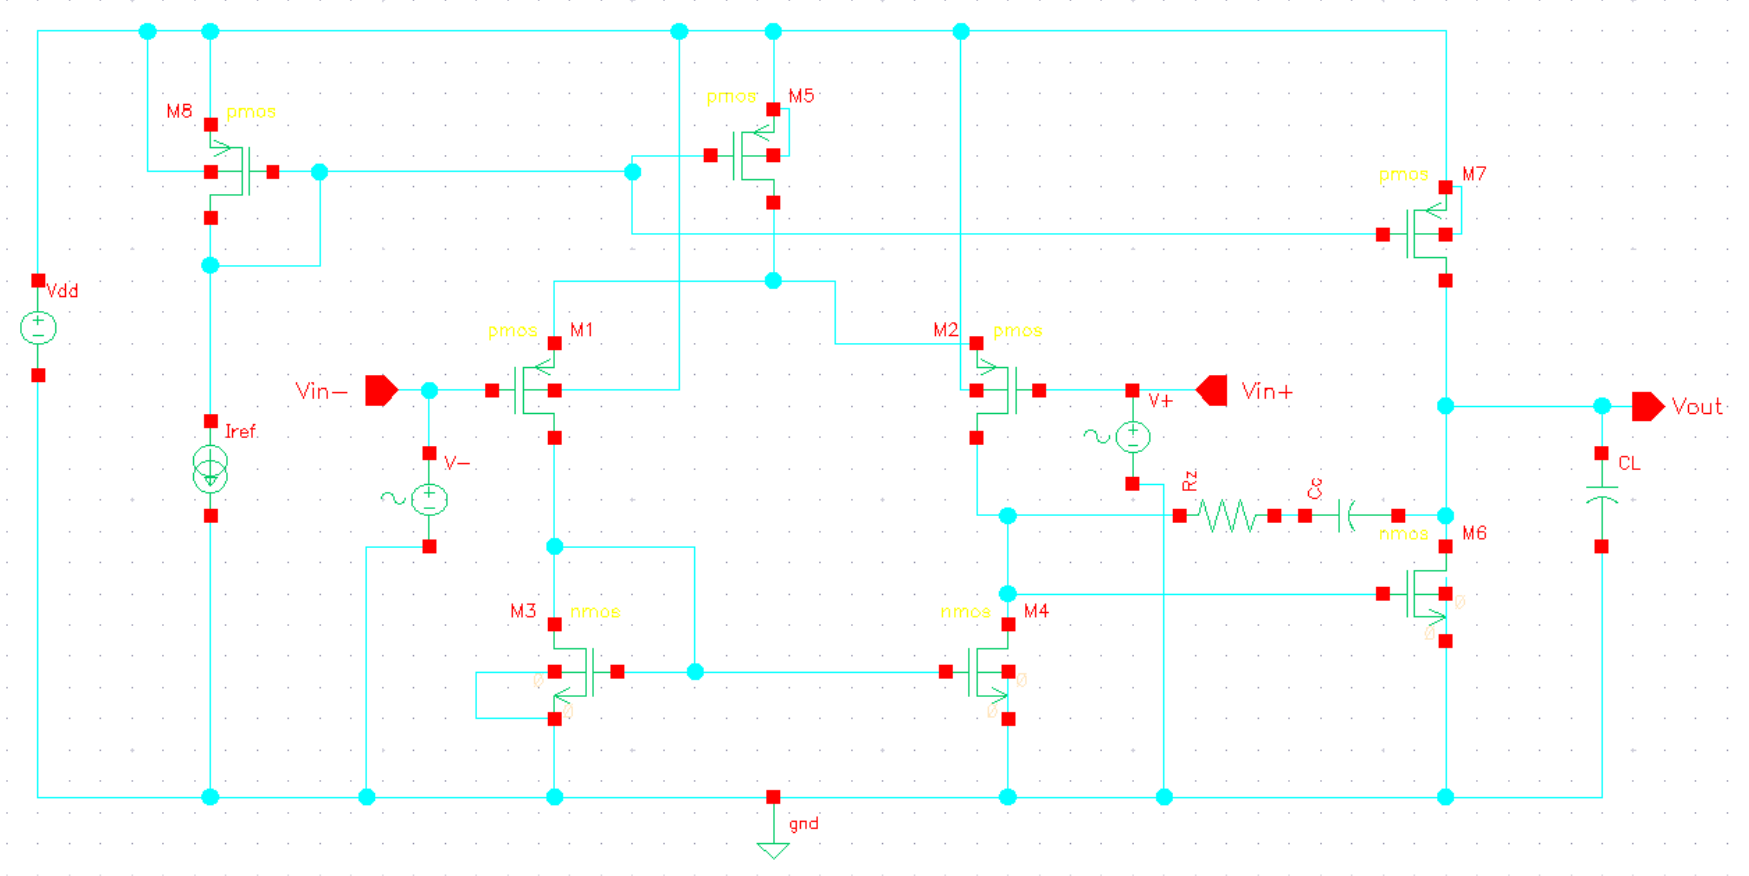
\includegraphics[width=\columnwidth]{fig_sch.png}
\caption{Cadence Virtuoso schematic of the two-stage amplifier (gpdk180):
PMOS input pair M1/M2, NMOS mirror load M3/M4, PMOS bias mirror M8/M5/M7 from
$I_{ref}$, common-source second stage M6 with PMOS load M7, and $R_Z$--$C_C$
Miller network from the first-stage output to $V_{out}$; $C_L$ models the
load.}
\label{fig:sch}
\end{figure}

The input pair M1/M2 is PMOS. With a \SI{0.5}{\volt} common mode an NMOS pair
would not remain in saturation --- its required minimum common mode (tail
overdrive plus $V_{TH}$ plus input overdrive) exceeds \SI{0.5}{\volt} ---
whereas a PMOS pair referenced to the \SI{1.8}{\volt} rail senses low
common-mode inputs naturally; PMOS inputs also exhibit lower $1/f$ noise,
which matters for the low-frequency biomedical-class loads the project
targets \cite{razavi}. The NMOS mirror M3/M4 converts the differential
current to a single-ended signal at the M4 drain; M8 is the diode-connected
master of the PMOS bias mirror fed by $I_{ref}$, with M5 supplying the
\SI{1}{\micro\ampere} tail and M7 the second-stage load current. M6 forms a
common-source second stage, giving the output swing needed to drive a PMOS
pass gate. Stability is set by pole splitting through $C_C$ with series
resistor $R_Z \approx 1/g_{m6}$ to cancel the RHP zero \cite{gray,allen}. The
exact $C_C$, $R_Z$ and $C_L$ component values are not visible in the supplied
schematic captures and must be confirmed from the schematic properties:
\textbf{[INSERT VERIFIED $C_C$/$R_Z$/$C_L$ FROM CADENCE]}.

\subsection{Hand sizing}
Devices were sized with the square-law expression, using the first-order
gpdk180 stand-in constants $k_n = \mu_n C_{ox} =
\SI{316}{\micro\ampere\per\volt\squared}$ and $k_p =
\SI{62.5}{\micro\ampere\per\volt\squared}$ taken from the reference paper's
device table \cite{patel2017}:
\begin{equation}
\frac{W}{L} = \frac{2 I_D}{k \, V_{ov}^2}
\label{eq:wl}
\end{equation}
where $I_D$ is the branch drain current and $V_{ov} = V_{GS}-V_{TH}$ the
chosen overdrive. Overdrives of \SI{0.12}{\volt} (input pair, maximizing
$g_m/I_D$), \SI{0.15}{\volt} (NMOS mirror and M6) and \SI{0.20}{\volt} (PMOS
current sources) give the sizing of Table~\ref{tab:size}.
Equation~\eqref{eq:wl} is an idealized long-channel approximation: the final
operating point must come from simulation, and Section~VII quantifies where
it deviates.

\begin{table}[!t]
\caption{Transistor Sizing (From the Project's Calculated Table)}
\label{tab:size}
\centering\footnotesize
\begin{tabular}{@{}llllllll@{}}
\toprule
Device & Type & $I_D$ & $V_{ov}$ & $W/L$ & $W$ & $L$ & Rationale \\
 & & (\si{\micro\ampere}) & (V) & calc & (\si{\micro\metre}) & (\si{\micro\metre}) & \\
\midrule
M1, M2 & PMOS & 0.5 & 0.12 & 1.11 & 1.1 & 1 & Input pair; low $V_{ov}$ \\
M3, M4 & NMOS & 0.5 & 0.15 & 0.14 & 0.4 & 2.855 & Mirror; long $L$ \\
M5 & PMOS & 1.0 & 0.20 & 0.80 & 0.8 & 1 & Tail (M8 $\times$1) \\
M6 & NMOS & 2.0 & 0.15 & 0.56 & 0.56 & 1 & CS; $V_{ov}$ matches M3/M4 \\
M7 & PMOS & 2.0 & 0.20 & 1.60 & 1.6 & 1 & Load (M8 $\times$2) \\
M8 & PMOS & 1.0 & 0.20 & 0.80 & 0.8 & 1 & Bias diode, $I_{ref}$=\SI{1}{\micro\ampere} \\
\bottomrule
\end{tabular}
\end{table}

\subsection{Small-signal design relations}
The first-stage gain, second-stage gain, unity-gain bandwidth and slew rate
obey the standard two-stage relations \cite{gray,allen}:
\begin{align}
A_{v1} &= g_{m1}\,(r_{o2}\,\|\,r_{o4}) \label{eq:av1}\\
A_{v2} &= g_{m6}\,(r_{o6}\,\|\,r_{o7}) \label{eq:av2}\\
\mathrm{GBW} &= \frac{g_{m1}}{2\pi C_C} \label{eq:gbw}\\
\mathrm{SR} &= \frac{I_{tail}}{C_C} \label{eq:sr}
\end{align}
where $g_{mi}$ and $r_{oi}$ are the transconductance and output resistance of
device M$i$, $C_C$ the Miller capacitor and $I_{tail}$ the tail current. With
the simulated $g_{m1} = \SI{6.43}{\micro\siemens}$ and the measured GBW of
\SI{1.629}{\mega\hertz}, \eqref{eq:gbw} implies an effective compensation
capacitance of about \SI{0.63}{\pico\farad}; this is a consistency check
derived from measured values, not a design entry, and the drawn $C_C$ must
still be read from the schematic.

\section{Simulation Methodology}
All simulations ran in the Cadence Analog Design Environment (ADE) with the
Spectre engine on gpdk180 models, $V_{DD}=\SI{1.8}{\volt}$,
$I_{ref}=\SI{1}{\micro\ampere}$ and \SI{27}{\celsius}, as evidenced by the
ADE session captures. The recorded analyses are: (i) a DC operating point
with on-schematic annotation to confirm every device in saturation
(region~2); (ii) an AC sweep (\SI{10}{\hertz}--\SI{1}{\giga\hertz}) of the
differential gain for DC gain, $-3$~dB bandwidth and unity-gain frequency;
(iii) phase of the same response at the unity-gain frequency for phase
margin; (iv) a CMRR measurement computed as
$20\log_{10}[(V_{out}/V_{in+})/(V_{out,cm}/V_{cm})]$ using a replica bench
driven by a common-mode source; (v) a transient run (\SI{10}{\milli\second},
$\pm$\SI{1}{\milli\volt} differential sine at the \SI{0.5}{\volt} common
mode) and a \SI{2}{\milli\second} transient from which ADE's slewRate
function reports \SI{611.877}{\kilo\volt\per\second}; and (vi) an ADE output
named Power that reports \SI{4.7345}{\micro\watt}. The expression behind that
Power output is not visible in the captures, so its definition --- and in
particular whether it averages over a supply sweep that was active in the
same session --- requires confirmation: \textbf{[CONFIRM ADE POWER
EXPRESSION]}. Analyses not evidenced (PSRR, noise, corners, Monte Carlo,
post-layout) were not performed. Closing the LDO will additionally require
input-line and load sweeps, loop-gain (stability) analysis with the
\SI{10}{\micro\farad} output capacitor and its ESR, start-up transients and
PSRR \cite{rincon1998}.

\section{Results and Discussion}
\begin{figure}[!t]
\centering
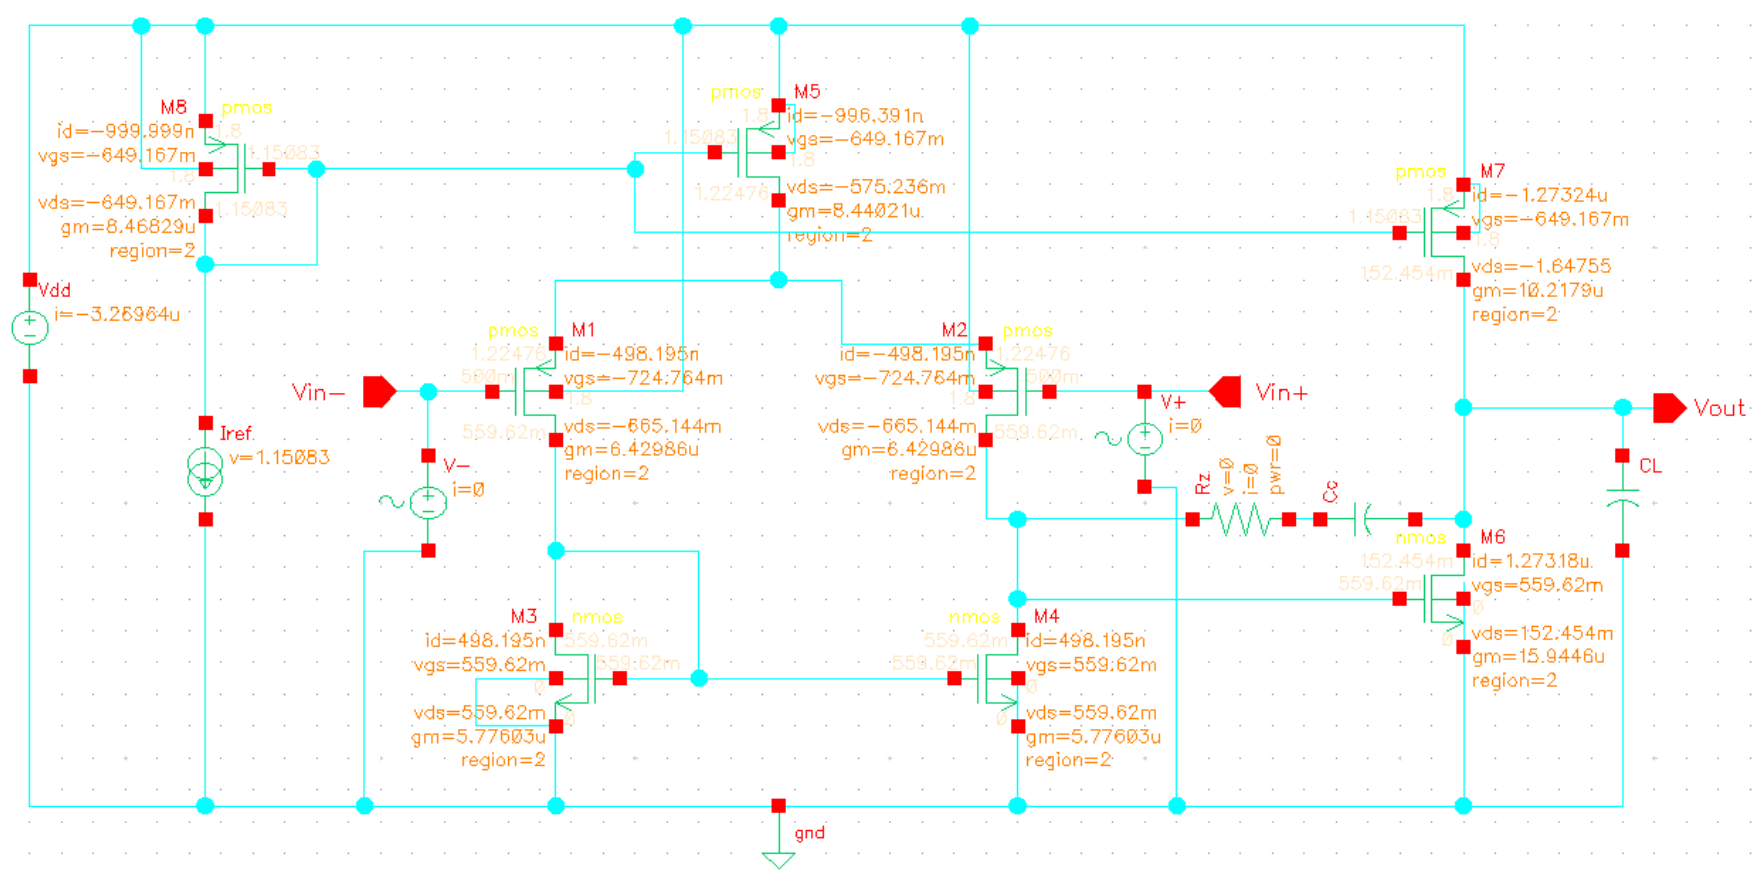
\includegraphics[width=\columnwidth]{fig_dcop.png}
\caption{DC operating point annotated on the schematic: every device reports
region~2 (saturation); supply current $i(V_{DD})=\SI{3.26964}{\micro\ampere}$;
tail devices carry $\approx$\SI{0.996}{\micro\ampere} and the second stage
\SI{1.273}{\micro\ampere}.}
\label{fig:dcop}
\end{figure}

\subsection{Operating point}
Table~\ref{tab:dcop} extracts the annotated operating point. All eight
transistors sit in saturation, validating the bias chain: M8 and M5 mirror
$I_{ref}$ accurately (0.996--1.0~\si{\micro\ampere}) and the pair splits the
tail evenly (\SI{0.498}{\micro\ampere} each). Two deviations from the hand
design deserve note. First, the second-stage current is
\SI{1.273}{\micro\ampere} rather than the intended \SI{2}{\micro\ampere} (a
$-36\,\%$ deviation), so the total supply current is \SI{3.27}{\micro\ampere}
instead of the planned \SI{4}{\micro\ampere}; the $W_7/W_8=2$ mirror ratio is
not realized exactly at this operating point, which first-order sizing with
assumed $k_p$ and channel-length modulation at $|V_{DS}|=\SI{1.65}{\volt}$
readily explains. Second, the open-loop output node rests at approximately
\SI{0.15}{\volt} ($V_{DS}$ of M6), far from mid-rail --- expected for an
uncommitted high-gain amplifier, and a reminder that this bench fixes the
bias only; in the LDO the feedback loop will place the output where the pass
device requires.

\begin{table}[!t]
\caption{DC Operating Point (From the Annotated Schematic, Fig.~\ref{fig:dcop})}
\label{tab:dcop}
\centering\footnotesize
\begin{tabular}{@{}lllllll@{}}
\toprule
Device & $I_D$ & $V_{GS}$ & $V_{DS}$ & $g_m$ & Region & Note \\
 & (\si{\micro\ampere}) & (mV) & (mV) & (\si{\micro\siemens}) & & \\
\midrule
M1/M2 & $-0.498$ & $-724.8$ & $-665.1$ & 6.43 & 2 & Balanced pair \\
M3/M4 & 0.498 & 559.6 & 559.6 & 5.78 & 2 & 1:1 mirror load \\
M5 & $-0.996$ & $-649.2$ & $-575.2$ & 8.44 & 2 & Tail $\approx I_{ref}$ \\
M6 & 1.273 & 559.6 & 152.5 & 15.94 & 2 & Output rests low \\
M7 & $-1.273$ & $-649.2$ & $-1648$ & 10.22 & 2 & $-36\,\%$ vs design \\
M8 & $-1.000$ & $-649.2$ & $-649.2$ & 8.47 & 2 & $V(I_{ref})=\SI{1.151}{\volt}$ \\
\bottomrule
\end{tabular}
\end{table}

\subsection{Frequency response, stability, CMRR}
\begin{figure}[!t]
\centering
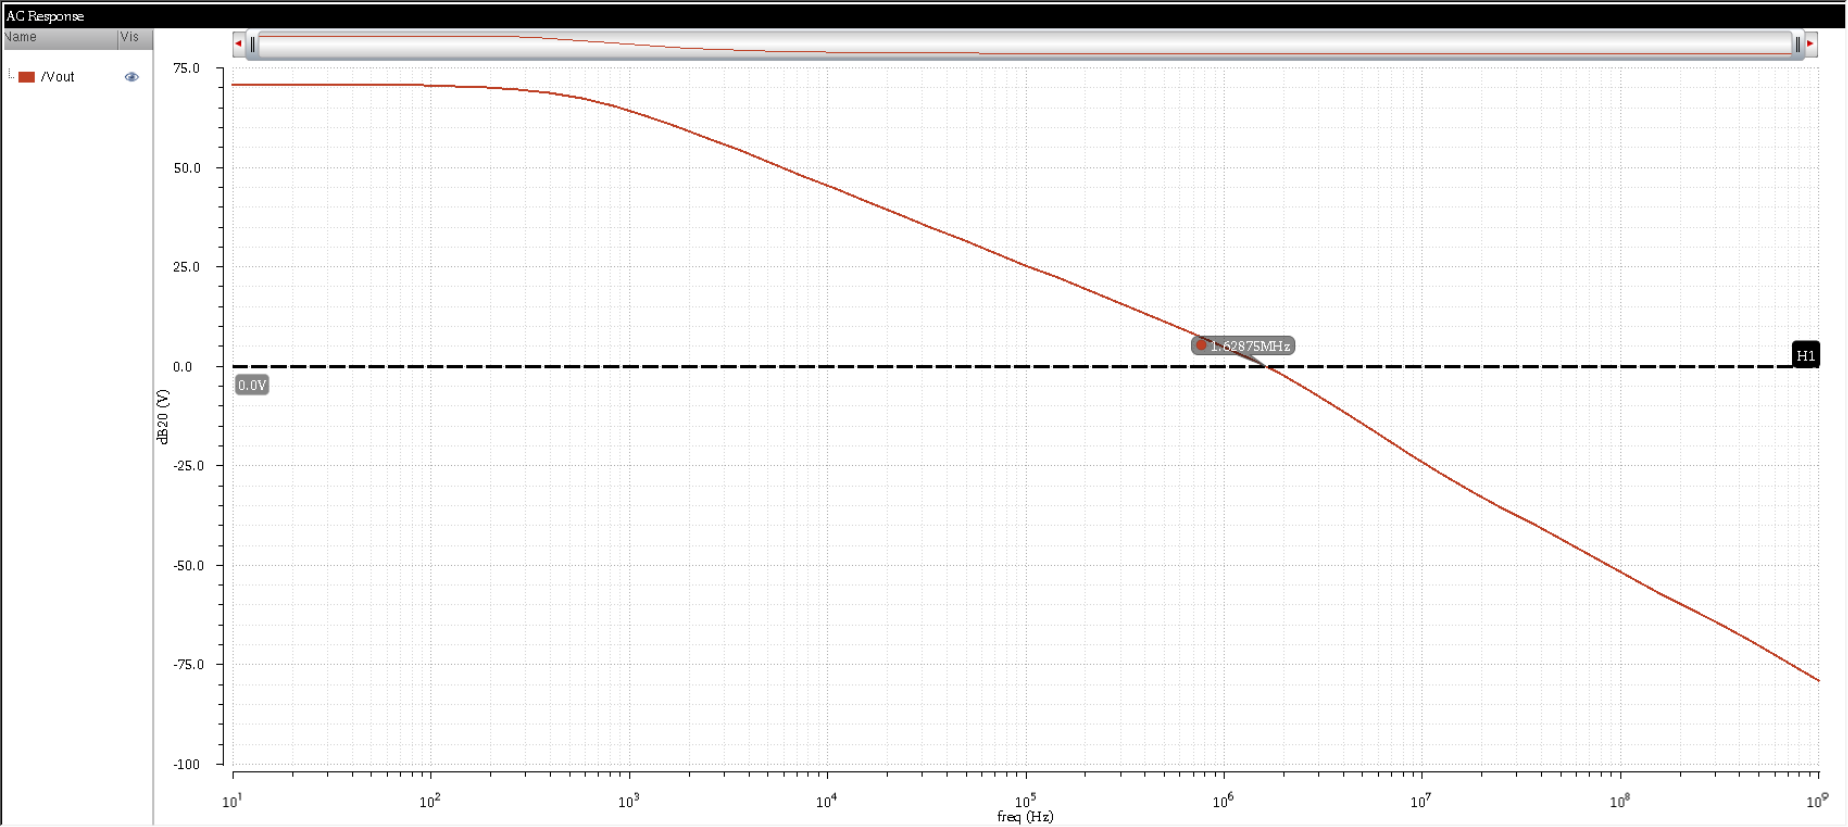
\includegraphics[width=0.92\columnwidth]{fig_gain.png}
\caption{Open-loop magnitude response: $\approx$\SI{70.5}{\decibel}
low-frequency gain; marker at the \SI{0}{\decibel} crossing gives a
unity-gain bandwidth of \SI{1.62875}{\mega\hertz}. A separate marker at
gain$-3$~dB (\SI{67.5}{\decibel}) gives the $-3$~dB bandwidth of
\SI{550.915}{\hertz}.}
\label{fig:gain}
\end{figure}
\begin{figure}[!t]
\centering
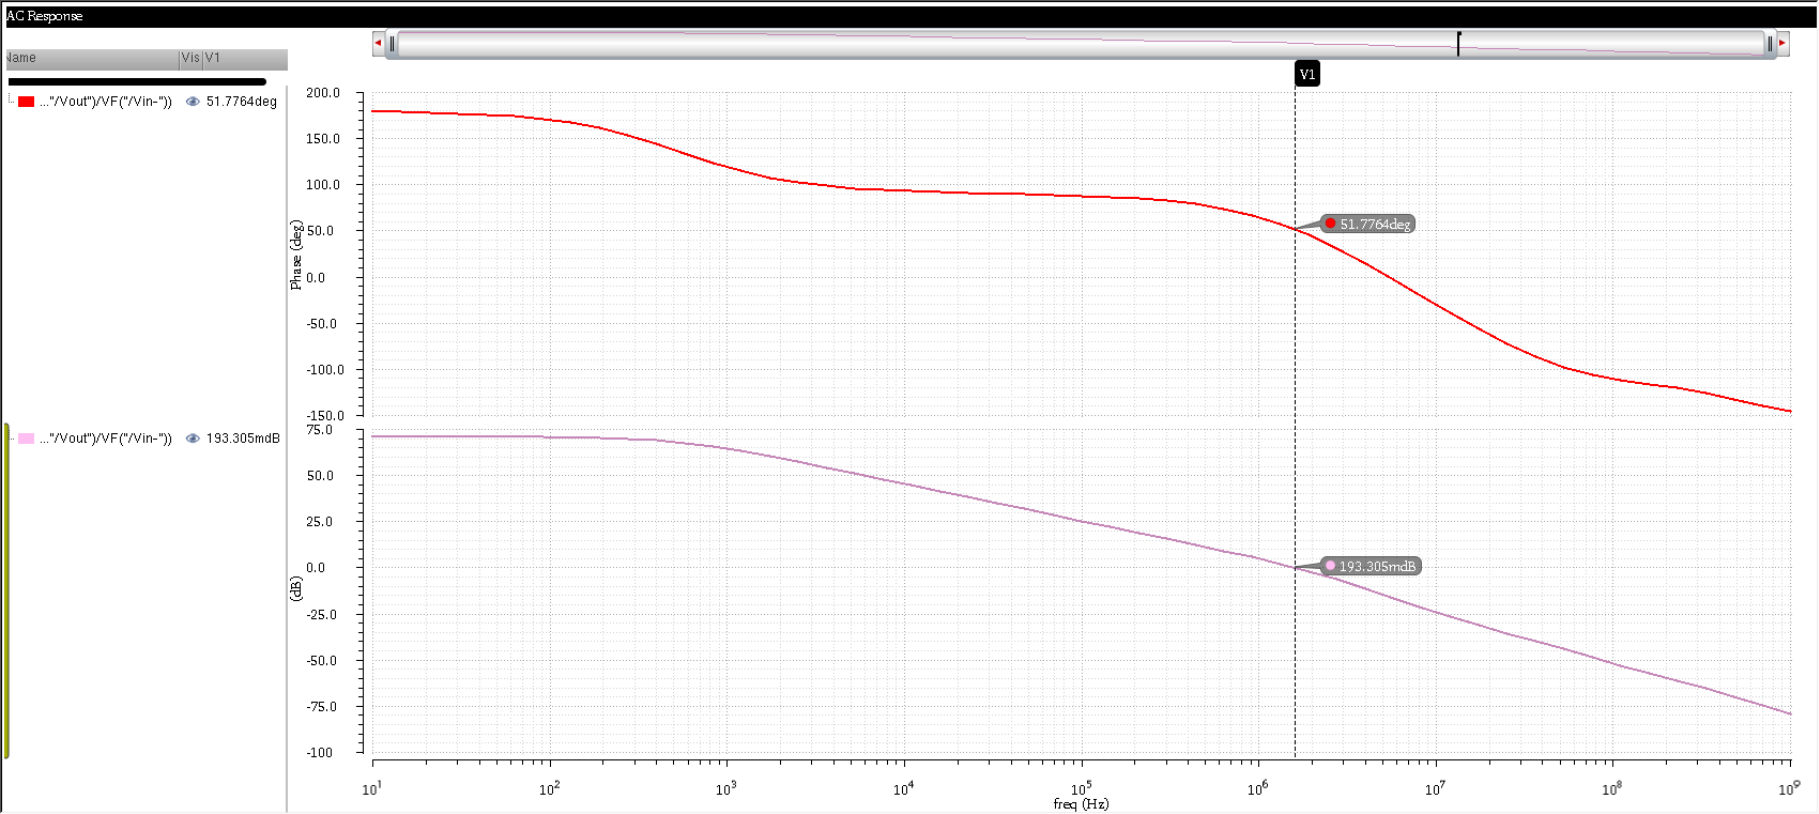
\includegraphics[width=0.92\columnwidth]{fig_pm.png}
\caption{Phase (top) and magnitude (bottom) at the unity-gain frequency: the
phase marker reads \ang{51.7764} where the gain is \SI{0.193}{\decibel},
i.e.\ a phase margin of $\approx$\ang{51.8}.}
\label{fig:pm}
\end{figure}

The amplifier reaches \SI{70.5}{\decibel} of DC gain --- inside the
60--80~dB target band --- with a single dominant pole at
$\approx$\SI{551}{\hertz} and a \SI{0}{\decibel} crossing at
\SI{1.629}{\mega\hertz}, consistent with a gain-bandwidth product of
$A_v \cdot f_{-3\mathrm{dB}} \approx 3350 \times \SI{551}{\hertz} \approx
\SI{1.85}{\mega\hertz}$ to first order. The phase margin is approximately
\ang{51.8}. This is a genuine shortfall against the \ang{60} guideline
adopted at specification time (the presentation's final table relaxes the
target to 45--\ang{60}): \ang{51.8} is stable and acceptable for initial
characterization, but a two-stage amplifier destined for an LDO loop ---
where the pass device and output capacitor add further phase lag --- should
enter that loop with margin in hand. Increasing $C_C$, retuning $R_Z$ toward
$1/g_{m6}$, or accepting a lower GBW are the standard remedies \cite{gray};
this retuning is scheduled before loop closure rather than claimed complete.

\begin{figure}[!t]
\centering
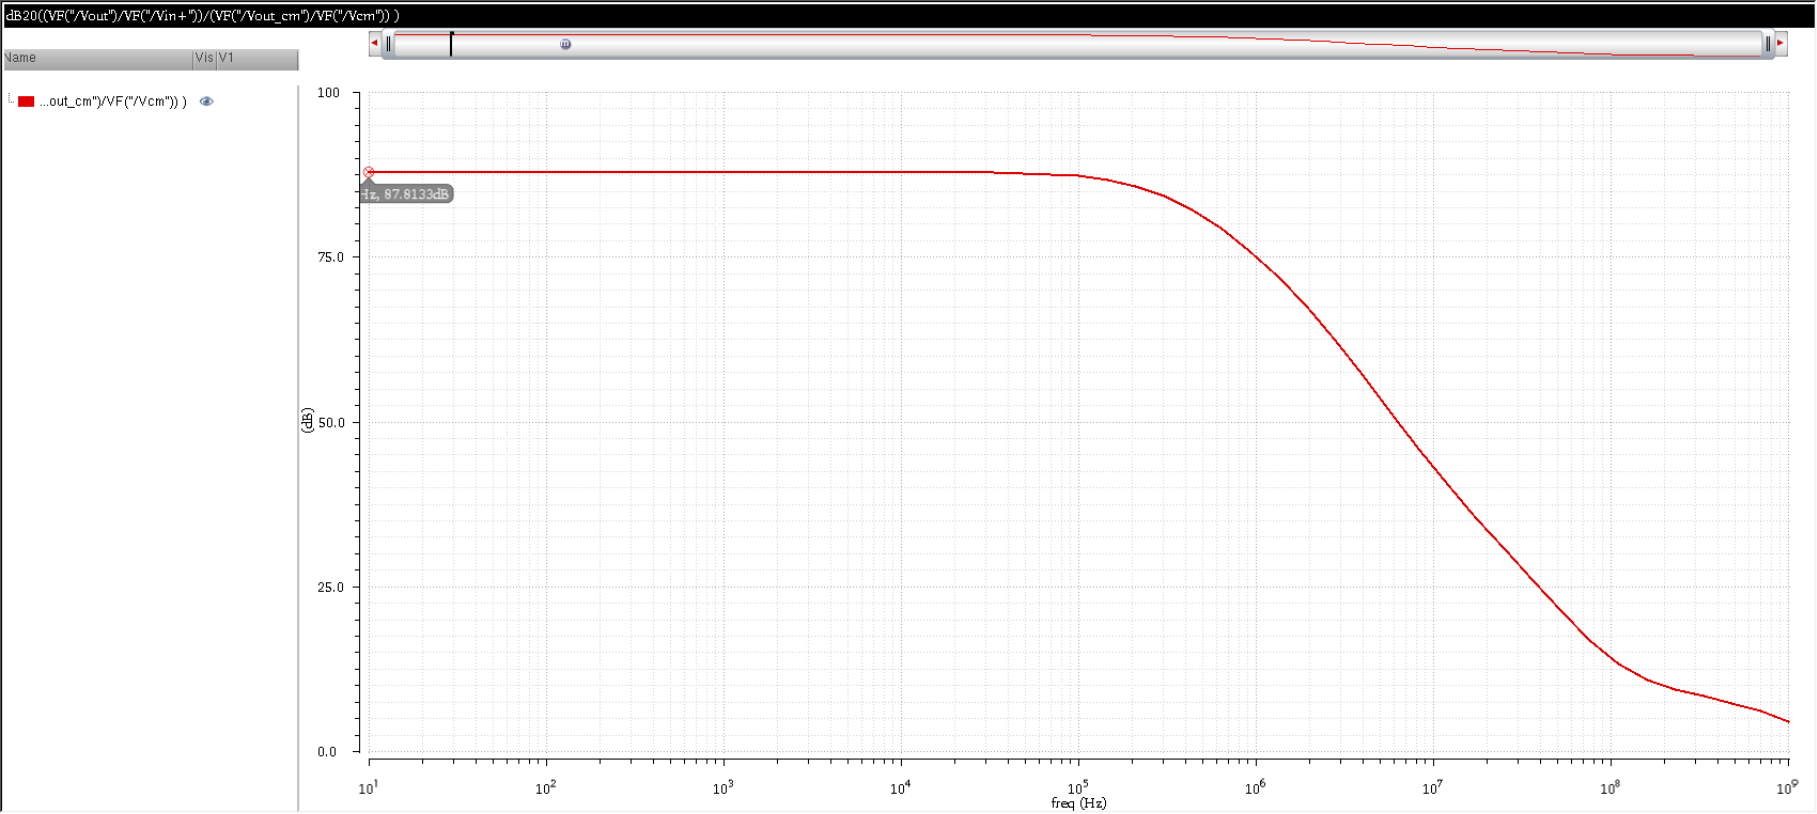
\includegraphics[width=0.92\columnwidth]{fig_cmrr.png}
\caption{CMRR versus frequency computed as
$20\log_{10}[(V_{out}/V_{in+})/(V_{out,cm}/V_{cm})]$: \SI{87.8133}{\decibel}
at \SI{10}{\hertz}, flat through the audio band and rolling off beyond
$\approx$\SI{100}{\kilo\hertz}.}
\label{fig:cmrr}
\end{figure}

\subsection{Transient behaviour and power}
\begin{figure}[!t]
\centering
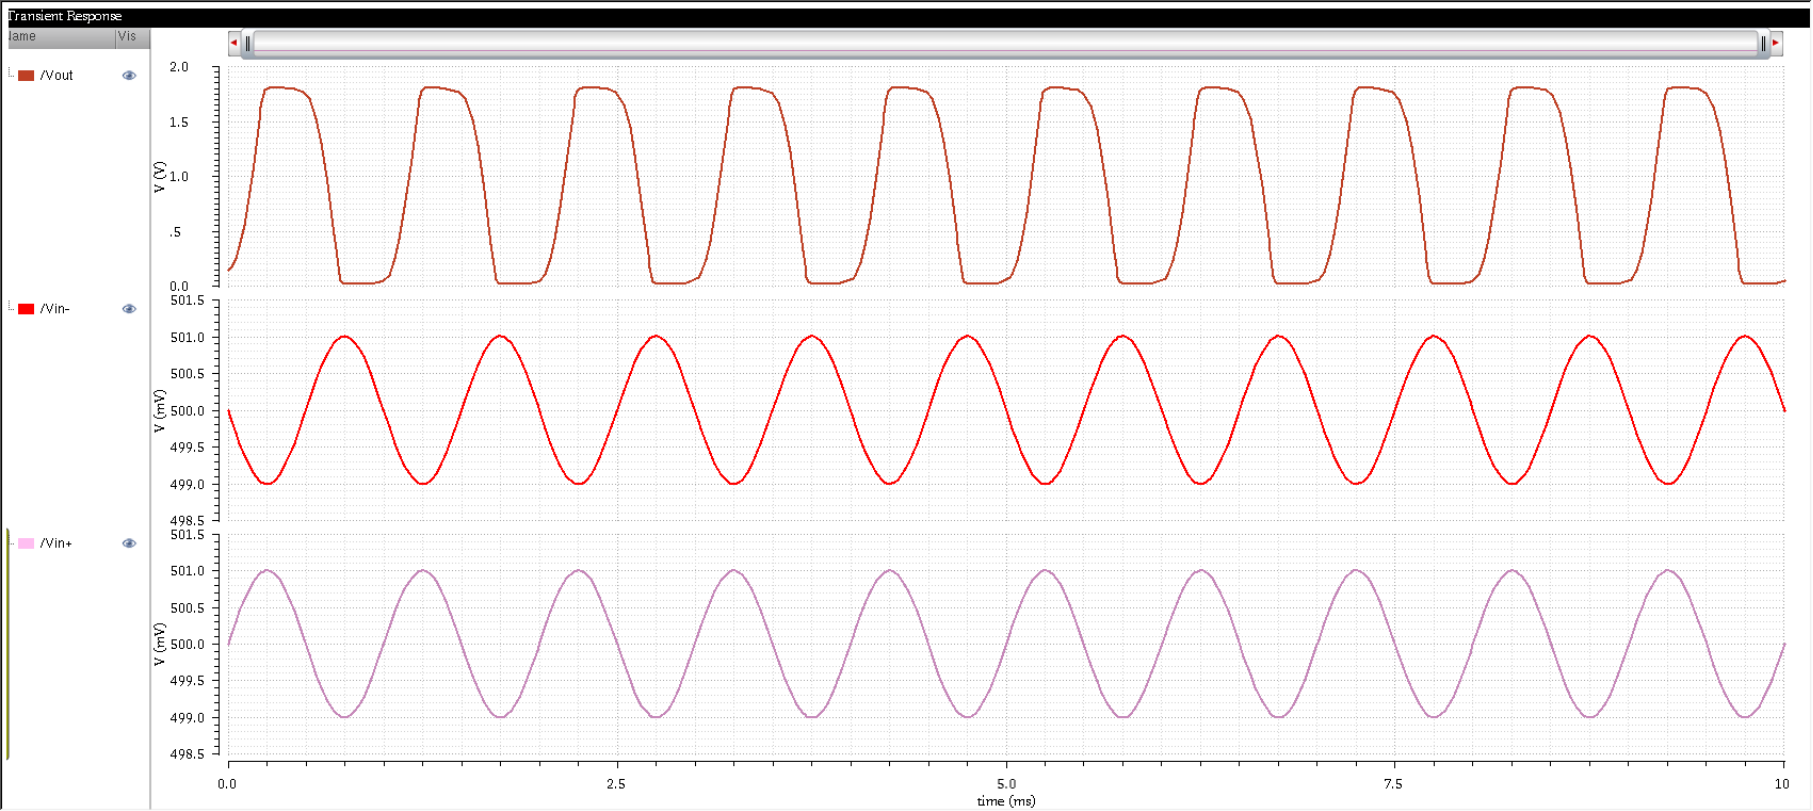
\includegraphics[width=0.92\columnwidth]{fig_tran.png}
\caption{Open-loop transient with a $\pm$\SI{1}{\milli\volt},
$\approx$\SI{1}{\kilo\hertz} differential drive about the \SI{0.5}{\volt}
common mode: the \SI{70.5}{\decibel} gain saturates the output, which swings
essentially rail to rail ($\approx$0.05--\SI{1.8}{\volt}).}
\label{fig:tran}
\end{figure}

Fig.~\ref{fig:tran} is an open-loop test: a millivolt-level input times
$\approx$3350~V/V exceeds the supply, so the output clips; the waveform
demonstrates polarity, swing and absence of latch-up, and is not an LDO
load-step response. The ADE slewRate output on a dedicated
\SI{2}{\milli\second} transient reports \SI{611.877}{\kilo\volt\per\second}
$\approx \SI{0.612}{\volt\per\micro\second}$, meeting the
$\ge$\SI{0.1}{\volt\per\micro\second} target. For power, two numbers coexist
in the evidence and must not be conflated: the ADE output reports
\SI{4.7345}{\micro\watt} (definition unconfirmed, Section~VI), while the DC
operating point implies
\begin{equation}
P = V_{DD} \cdot I_{DD} = \SI{1.8}{\volt} \times \SI{3.26964}{\micro\ampere}
  \approx \SI{5.885}{\micro\watt}.
\label{eq:power}
\end{equation}
Both lie comfortably inside the ${<}10$--\SI{100}{\micro\watt} budget, but
the $\approx$20\,\% gap between them is a measurement-definition question,
not a physical result, and is flagged for resolution. Table~\ref{tab:res}
assembles the verified results.

\begin{table}[!t]
\caption{Amplifier Simulation Results (Standalone, gpdk180, \SI{1.8}{\volt})}
\label{tab:res}
\centering\footnotesize
\begin{tabular}{@{}llllll@{}}
\toprule
Parameter & Target & Simulated & Unit & Assessment & Evidence \\
\midrule
DC open-loop gain & 60--80 & $\approx$70.5 & dB & Met & Fig.~\ref{fig:gain} \\
$-3$ dB bandwidth & --- & 550.915 & Hz & Consistent & Fig.~\ref{fig:gain} \\
Unity-gain bandwidth & 0.01--2 & 1.62875 & MHz & Met & Fig.~\ref{fig:gain} \\
Phase margin & $\ge$60 (45--60) & $\approx$51.8 & deg & Below \ang{60} & Fig.~\ref{fig:pm} \\
CMRR @ 10 Hz & 80--100 & 87.8133 & dB & Met & Fig.~\ref{fig:cmrr} \\
Slew rate & $\ge$0.1--1 & $\approx$0.612 & V/\si{\micro\second} & Met & ADE output \\
Supply current & --- & 3.26964 & \si{\micro\ampere} & --- & Fig.~\ref{fig:dcop} \\
Power (ADE) & $<$10--100 & 4.7345 & \si{\micro\watt} & Met; def.\ pending & ADE capture \\
Power ($V_{DD}I_{DD}$) & $<$10--100 & $\approx$5.885 & \si{\micro\watt} & Met; \eqref{eq:power} & Fig.~\ref{fig:dcop} \\
PSRR, noise, corners & --- & Not measured & --- & Pending & --- \\
\bottomrule
\end{tabular}
\end{table}

\section{Proposed LDO Implementation and Verification Plan}
The amplifier connects into the LDO without internal modification: its output
drives the gate of an external PMOS pass transistor whose source ties to the
LDO input rail, $V_{ref}=\SI{0.5}{\volt}$ drives the inverting input, and the
non-inverting input takes the feedback voltage from the $R_1$/$R_2$ divider
across the output. The divider sets the regulated output as
\begin{equation}
V_{out} = V_{ref}\left(1 + \frac{R_1}{R_2}\right)
\label{eq:div}
\end{equation}
so the proposed $R_1=\SI{700}{\kilo\ohm}$ and $R_2=\SI{500}{\kilo\ohm}$ with
a \SI{0.5}{\volt} reference give $V_{out}=0.5(1+1.4)=\SI{1.2}{\volt}$, with
$\approx$\SI{1}{\micro\ampere} standing divider current. The remaining
component proposals from the LDO implementation manual are listed in
Table~\ref{tab:ldo}; all are starting values for simulation, none is a
verified result. Note that the LDO implementation manual itself was not
present in the supplied evidence folder; its values are reproduced from the
project brief and must be cross-checked against the manual before submission.
Table~\ref{tab:vm} defines the verification matrix the LDO must pass; the
large \SI{10}{\micro\farad} output capacitor and its \SI{16}{\ohm} ESR
dominate loop dynamics and will interact with the amplifier's \ang{51.8}
margin, which is precisely why loop-gain simulation precedes any performance
claim \cite{rincon1998}.

\begin{table}[!t]
\caption{Proposed LDO Components (Starting Values --- Not Simulated Results)}
\label{tab:ldo}
\centering\footnotesize
\begin{tabular}{@{}llll@{}}
\toprule
Component & Proposed value & Purpose & Status \\
\midrule
Nominal LDO input & \SI{1.8}{\volt} & Supply at closure & Pending \\
Target output & \SI{1.2}{\volt} & Regulated rail & Pending \\
Reference voltage & \SI{0.5}{\volt} & Set-point for \eqref{eq:div} & Pending \\
Max load current & \SI{100}{\micro\ampere} & Load envelope & Pending \\
PMOS pass device & $W$=\SI{60}{\micro\metre}, $L$=\SI{0.5}{\micro\metre} & Low-dropout source & Pending \\
$R_1$ / $R_2$ & 700 / \SI{500}{\kilo\ohm} & Divider, \eqref{eq:div} & Pending \\
Output capacitor & \SI{10}{\micro\farad} & Hold-up, load pole & Pending \\
Capacitor ESR & \SI{16}{\ohm} & ESR zero & Pending \\
\bottomrule
\end{tabular}
\end{table}

\begin{table}[!t]
\caption{LDO Verification Matrix (All Items Currently: Not Measured)}
\label{tab:vm}
\centering\footnotesize
\begin{tabular}{@{}llll@{}}
\toprule
Test & Conditions & Quantity & Acceptance \\
\midrule
DC closure & $V_{IN}$=\SI{1.8}{\volt}, no load & $V_{out}$, regions & \SI{1.2}{\volt}; all sat. \\
Line sweep & $V_{IN}$ swept & $\Delta V_{out}/\Delta V_{IN}$ & Spec to be set \\
Load sweep & 0$\to$\SI{100}{\micro\ampere} & $\Delta V_{out}/\Delta I_L$ & Spec; dropout noted \\
Loop gain & $C_{out}$=\SI{10}{\micro\farad}, ESR \SI{16}{\ohm} & PM, GM & PM $\ge$ \ang{45} \\
Load/line step & Step $I_L$, $V_{IN}$ & Over/undershoot & No oscillation \\
Start-up & $V_{IN}$ ramp & $V_{out}$ trajectory & Monotonic \\
PSRR & AC on $V_{IN}$ & $V_{out}/V_{IN}(f)$ & Spec to be set \\
\bottomrule
\end{tabular}
\end{table}

\section{Limitations and Future Work}
Observed limitations from the evidence: the \ang{51.8} phase margin; the
second-stage current and mirror-ratio deviation; the open-loop-only transient
characterization; the unresolved power-measurement definition; and the
standalone testbench operating point (ideal \SI{1.8}{\volt} supply, output
resting near \SI{0.15}{\volt}). Anticipated --- but not yet observed ---
challenges concern the system: start-up from a weak 0.3--1~\si{\volt} source,
headroom for the amplifier and pass device when the stored rail sags,
reference accuracy at low voltage, quiescent-current budget once all blocks
are active, loop stability with the \SI{10}{\micro\farad}/\SI{16}{\ohm}
output network, output ripple under duty-cycled loads, and the absence of
corner, mismatch and post-layout verification. Table~\ref{tab:lim} ranks
these with remedies; the prioritized plan is: (1) confirm the power
definition, $C_C$/$R_Z$/$C_L$ values and re-tune the compensation to
$\ge$\ang{60}; (2) close and DC-verify the LDO; (3) loop-gain and transient
verification with the output network; (4) implement the \SI{0.5}{\volt}
reference \cite{seok2012}; (5) design the conditioning/boost stage and
storage \cite{seeman2008}; (6) add the voltage monitor and load switch;
(7) full-PMU simulation under varying input and load; (8) PVT, mismatch and
post-layout checks as tools permit.

\begin{table}[!t]
\caption{Limitations and Future Work}
\label{tab:lim}
\centering\footnotesize
\begin{tabular}{@{}llll@{}}
\toprule
Issue & Impact & Remedy & Priority \\
\midrule
PM \ang{51.8} $<$ \ang{60} (observed) & Risk in LDO loop & Increase $C_C$/retune $R_Z$ & High \\
2nd-stage $-36\,\%$ (observed) & Lower SR/$A_{v2}$ & Re-size M7 or re-document & Medium \\
Power def.\ unconfirmed (observed) & 4.73 vs 5.89~\si{\micro\watt} & Explicit $V_{DD}I$ expression & High \\
Open-loop transient only (observed) & No settling data & Unity-gain / LDO benches & High \\
Harvester headroom (anticipated) & Cannot feed LDO & Boost/SC stage \cite{seeman2008} & High \\
Reference accuracy (anticipated) & Set-point error & Dedicated design \cite{seok2012} & Medium \\
No PVT/post-layout (gap) & Unquantified spread & Corners, MC, extraction & Medium \\
\bottomrule
\end{tabular}
\end{table}

\section{Conclusion}
This work set out the architecture of a solar energy-harvesting PMU and
completed, at schematic level in 0.18~\si{\micro\metre} CMOS, its central
analog block: a two-stage, PMOS-input, Miller-compensated error amplifier
intended for the PMU's LDO. Square-law hand sizing carried the design to a
bias point that simulation confirms device by device, and the standalone
characterization yields \SI{70.5}{\decibel} gain, \SI{1.629}{\mega\hertz}
unity-gain bandwidth, \SI{87.8}{\decibel} CMRR,
$\approx$\SI{0.612}{\volt\per\micro\second} slew rate and microwatt-level
power from a \SI{1.8}{\volt} supply --- figures compatible with its role as
an LDO error amplifier. The characterization is equally clear about what is
not yet achieved: the \ang{51.8} phase margin must be raised before loop
closure, the power-measurement definition needs confirmation, and the LDO,
reference, conditioning stage, storage and monitor exist only as a specified
plan with starting component values. The next milestone --- closing the LDO
around the unchanged amplifier and verifying regulation and loop stability
against Table~\ref{tab:vm} --- will convert the proposed PMU from an
architecture into a demonstrated system.

\begin{thebibliography}{7}
\bibitem{patel2017}
P.~Patel, B.~Mishra, and D.~Nagchoudhuri, ``A 36 nW power management unit for
solar energy harvesters using 0.18~\si{\micro\metre} CMOS,'' in \emph{Proc.
IEEE Int. Symp. VLSI Design and Test (VDAT)}, 2017.
\bibitem{rincon1998}
G.~A. Rinc\'on-Mora and P.~E. Allen, ``A low-voltage, low quiescent current,
low drop-out regulator,'' \emph{IEEE J. Solid-State Circuits}, vol.~33,
no.~1, pp. 36--44, Jan. 1998.
\bibitem{razavi}
B.~Razavi, \emph{Design of Analog CMOS Integrated Circuits}, 2nd~ed. New
York, NY, USA: McGraw-Hill, 2017.
\bibitem{gray}
P.~R. Gray, P.~J. Hurst, S.~H. Lewis, and R.~G. Meyer, \emph{Analysis and
Design of Analog Integrated Circuits}, 5th~ed. Hoboken, NJ, USA: Wiley, 2009.
\bibitem{allen}
P.~E. Allen and D.~R. Holberg, \emph{CMOS Analog Circuit Design}, 3rd~ed.
New York, NY, USA: Oxford Univ. Press, 2012.
\bibitem{seok2012}
M.~Seok, G.~Kim, D.~Blaauw, and D.~Sylvester, ``A portable 2-transistor
picowatt temperature-compensated voltage reference operating at 0.5 V,''
\emph{IEEE J. Solid-State Circuits}, vol.~47, no.~10, pp. 2534--2545, Oct.
2012.
\bibitem{seeman2008}
M.~D. Seeman and S.~R. Sanders, ``Analysis and optimization of
switched-capacitor DC--DC converters,'' \emph{IEEE Trans. Power Electron.},
vol.~23, no.~2, pp. 841--851, Mar. 2008.
\end{thebibliography}

\end{document}
